\documentclass[main.tex]{subfiles}
\pagestyle{main}%%%
\begin{document}

\chapter{Préservation de l'invariance par rotation sur maillage cartésien \label{chap:trefle}}
%\vspace{-13mm}
%\begin{flushright}
%{ \Large\sf ou Vous avez dit trèfle à 4 feuilles ?\ }
%\end{flushright}

%\mylettrine{C}{e} chapitre aurait pu ce nommer \og Vous avez dit trèfle à 4 feuilles ? \fg{}, car oui en effet, comme nous allons le voir au début de ce chapitre, discrétiser notre modèle avec des schémas standards va produire une 
%
%\mylettrine{T}{ransporter} (ou diffuser) une quantité invariante par rotation n'est pas chose facile. Pour illustrer cela, nous allons montrer dans un premier temps les résultats obtenus, lorsqu'on discrétise le modèle présenté au chapitre précédent avec des schémas classiques.  Nous examinerons ensuite les diverses sources causant

\mylettrine{C}{onsidérons} le modèle que nous avons construit au chapitre précédent avec pour donnée initiale des densités invariantes par rotation. Le champ de vitesses (dont la divergence est  donnée par ces mêmes densités, \cf Eq.~\eqref{eq_darcy}) est donc invariant par rotation. Ainsi pour tout temps nos densités devraient être invariantes par rotation. Sauf que sur maillage cartésien, avec les schémas numériques classiques, pour certains jeux de paramètres,  cette propriété n'est pas du tout conservée au fil du temps... Comme nous allons le présenter au début de ce chapitre, les lignes de niveaux, au départ circulaires, vont peu à peu se déformer devenant progressivement carrées puis prenant plus tard la forme d'un trèfle à 4 feuilles !... Deux pistes seront alors étudiées~:
\begin{myitemize}
\item défaut du schéma de diffusion
\item défaut du schéma de transport
\end{myitemize}


\noindent Une fois le défaut identifié, un correctif sera finalement proposé~: le schéma \twinweno. 

\section{Présentation du problème}
Sans plus tarder, présentons le problème en image. Sur la Figure~\ref{fig:trefle}, est présentée une simulation numérique du modèle EDP construit au chapitre précédent avec~:
\begin{myitemize}
\item un schéma classique à 5 points pour la diffusion,
\item un WENO5 (avec splitting directionnel) pour le transport.
\end{myitemize}
\begin{figure}
\centering
  \subfloat[Jour 0]{\label{fig_chen_simu_spatial_1}
\includegraphics[width=0.33\textwidth]
{track_10x10_7/vue_S/1.png}}
\subfloat[Jour 543]{\label{fig_chen_simu_spatial_2}
\includegraphics[width=0.33\textwidth]
{track_10x10_7/vue_S/34.png}}
\subfloat[Jour 1053]{\label{fig_chen_simu_spatial_4}
\includegraphics[width=0.33\textwidth]
{track_10x10_7/vue_S/65.png}}
\caption{\label{fig:trefle} Simulations numériques réalisées avec un WENO5 pour le transport et un Laplacien classique à 5 points pour la diffusion. Partant d'une donnée initiale circulaire, 
une structure en forme de trèfle apparaît.}
\end{figure}

Partant d'une donnée initiale irrotationelle, on constate que la simulation numérique peut générer une structure en forme de trèfle, comme présentée  sur la Figure~\ref{fig:trefle}, alors que la forme circulaire devrait être préservée. 

Ce problème n'apparaît pas de manière systématique. L'ensemble des simulations numériques réalisées pour \Nber, ne le faisait pas apparaître. Le problème a été identifié par incident, lorsque nous cherchions à recoller notre modèle aux données de \Chen. 


Notez que ce type d'erreur sur la forme conduit à une erreur sur l'évolution de l'aire de la lésion. En effet la forme de trèfle augmente la surface de contact ce qui modifie l'interaction entre la vascularisation et la tumeur. Ce type d'instabilités doit être fixé.


\section{Le schéma de diffusion}
\subsection{Influence de la condition limite}
Le schéma associé à la diffusion a été le premier à être incriminé. En effet dans l'équation~\eqref{eq_pression_disc} sur la pression~$\Pi$, la condition limite (CL) est imposée au bord du domaine de calcul~$\Omega$, domaine qui est carré. La CL ne vérifie donc pas, dès le départ, l'invariance par rotation. Ceci est illustré sur la Figure~\ref{fig:ligne_nvx_laplace_carre} qui présente la solution de l'équation
\begin{equation}\label{eq:pression_iter1}
\left\{
\begin{aligned}
-\Delta \Pi(\vecx) &= P(t=0,x) & \quad \textrm{ dans }  \Omega , \\
\Pi(\vecx) &=0 & \quad \textrm{ sur  } \partial \Omega,
\end{aligned}
\right.
\end{equation}
qui n'est autre que l'équation résolue lors de la première itération de l'algorithme sur le modèle complet ($M$ étant initialisé au dessus du seuil d'hypoxie, on a alors au départ $\gammapp=1$ dans l'équation~\eqref{eq_darcy}. De plus, comme $N=0$ au départ, on obtient alors $\dive \vit = P$, car $k\equiv1$). Dans les itérations suivantes certes le second membre de l'équation va varier, mais cela ne va pas changer le fait que la forme du bord impacte les lignes de niveaux.
\begin{figure}
\centering
\subfloat[Sans masque\label{fig:ligne_nvx_laplace_carre} ]{
\includegraphics[width=.49\textwidth]
%{simu/trefle_track/point3_0/track_10x10_7/pression_2.png}
{simu/graph_v2.2.d/ref/pression_2.png}}
\subfloat[Avec un masque\label{fig:ligne_nvx_laplace_mask} ]{
\includegraphics[width=.49\textwidth]
%{simu/trefle_track/point3_0/track_10x10_7/pression_2.png}
{simu/graph_v2.2.d/ref_mask/pression_2.png}}
%\vspace{-4mm}\\
\caption{\label{fig:ligne_nvx_laplace} Résolution de la pression donnée par un laplacien. La forme du domaine de calcul carré se répercute sur le résultat.}
\end{figure}

L'effet carré sur les lignes de niveaux de la pression, apparaît surtout près du bord du domaine de calcul. Ainsi, pour tenter de palier à ce défaut, la première idée fut de considérer un domaine plus grand, laissant une sorte de couche limite pour absorber les déformations. Des simulations numériques de notre modèle ont été réalisées en doublant la longueur dans chaque direction (la taille d'une maille restant inchangée, on double aussi le nombre de mailles). Malheureusement, une forme de trèfle est toujours visible. On a même du mal à distinguer visuellement s'il y a eu une amélioration. 
%Visiblement cette 
Cette couche limite ne suffit donc pas. 
La seconde idée, fut d'imposer la CL sur un cercle, de sorte à ce que celle-ci soit invariante par rotation. Considérons alors un disque~$\mathcal{D}$ (un masque) inclus dans notre domaine de calcul initial~$\Omega$ et imposons la CL de Dirichlet sur son bord. L'équation~\eqref{eq_pression_disc} sur la pression devient alors~: 
\begin{equation}\label{eq:pression_iter1_mask}
\left\{
\begin{aligned}
-\Delta \Pi(t,\vecx) &= F(t,\vecx) & \quad \textrm{ dans }  \mathcal{D} , \\
\Pi(t,\vecx) &=0 & \quad \textrm{ sur  } \partial\mathcal{D},
\end{aligned}
\right. \quad \forall t>0
\end{equation}
Pour résoudre cela on procède par pénalisation de tout ce qui est à l'extérieur du disque~:
\begin{equation}\label{eq:pression_masque_penalisation}
- \Delta \Pi(t,\vecx) = F(t,\vecx) + \frac{1}{\epsilon} \Pi \mathds{1}_{\mathcal{D}^c}(\vecx),
\end{equation}
où $\mathcal{D}^c$ désigne le complémentaire de $\mathcal{D}$ et où $\epsilon$ est un paramètre de pénalisation (que l'on prend petit~: $10^-5$). Ainsi, le domaine de calcul reste~$\Omega$ entier, mais en dehors de~$\mathcal{D}$, la pénalisation impose\footnote{En multipliant l'équation~\eqref{eq:pression_masque_penalisation} par $\epsilon$ puis en faisant tendre $\epsilon$ vers 0, on obtient alors que la pénalisation impose $\Pi \mathds{1}_{\mathcal{D}^c}(\vecx)=0.$}~$\Pi=0$. Cette technique nous garantit ainsi l'invariance par rotation de~$\Pi$ si le terme source~$F$ l'est. 
Comme on peut le voir sur la Figure~\ref{fig:ligne_nvx_laplace_mask}, l'utilisation d'un masque permet bien d'assurer la préservation de l'invariance par rotation sur la pression. Malheureusement, les simulations numériques réalisées avec ce masque circulaire ne montrent qu'une très légère amélioration 
%\todo{Montrer graphique?} 
de la forme~: le trèfle persiste. 
Explorons alors une autre piste. 

\subsection{Schéma à 9 points}
La forme du trèfle fait très clairement apparaître les directions du maillage. Il est alors légitime de se demander si un schéma avec un stencil à 9 points ferait aussi apparaître ce genre de forme. 
\begin{figure}
\subfloat[\label{fig:schema_laplace_9pts_classique}Schéma classique]{
\resizebox{.49\textwidth}{!}{\setlength{\unitlength}{0.01\textwidth}
\begin{picture}(110,105)
%%\rect{0}{0}{110}{105}

\Huge
\squaremesh{10}{40}{2}
\multiput(10, 10)(0, 40){3}{\multiput(0, 0)(40, 0){3}{\circle*{5}}}

\put(12,3){%%% calque des legendes de noeuds
\multiput(0, 0)(0, 80){2}{\multiput(0, 0)(80, 0){2}{$-1$}}
\multiput(40, 0)(0, 80){2}{$-4$}
\multiput(0, 40)(80,0){2}{$-4$}
\put(40,40){$20$}
}
\put(85,95){\scalebox{2}{$\times \sfrac{1}{6h^2}$}}

\end{picture}
}}
\subfloat[\label{fig:schema_laplace_9pts_custom}Autre schéma découlant d'une méthode mixte VF/EF présentée dans l'annexe annexe~\ref{chap:anx_methode_mixte_VFEF}]{
\resizebox{.49\textwidth}{!}{\setlength{\unitlength}{0.01\textwidth}
\begin{picture}(110,105)
%%\rect{0}{0}{110}{105}

\Huge
\squaremesh{10}{40}{2}
\multiput(10, 10)(0, 40){3}{\multiput(0, 0)(40, 0){3}{\circle*{5}}}

\put(12,3){%%% calque des legendes de noeuds
\multiput(0, 0)(0, 80){2}{\multiput(0, 0)(80, 0){2}{$-1$}}
\multiput(40, 0)(0, 80){2}{$-2$}
\multiput(0, 40)(80,0){2}{$-2$}
\put(40,40){$12$}
}
\put(85,95){\scalebox{2}{$\times \sfrac{1}{4h^2}$}}

\end{picture}
}}
\caption{\label{fig:schema_laplacien}Poids associés à chacun des points du stencil à 9 points de schémas discrétisant le laplacien ($h$ étant le pas d'espace, égal dans chaque direction).}
\end{figure}
Le premier schéma à 9 points essayé est le schéma classique, présenté notamment dans~\cite{leveque2007finite}, ayant des poids comme indiqués sur la Figure~\ref{fig:schema_laplace_9pts_classique}. Aucune amélioration n'a malheureusement été constatée... Un second schéma à 9 points a été imaginé à partir d'une méthode mixte éléments finis/volumes finis comme présentée et utilisée dans~\cite{latige2013second}. Le principe est le suivant.  
%%%% Figure basculées en annexe
Sur chaque maille~$\mathcal{M}$, une approximation par un polynôme~$\mathbb{Q}1$ est réalisée à partir des valeurs aux quatre coins de la maille. Le flux au travers du volume de contrôle est alors calculé comme l'intégrale sur le bord de ce volume, de la dérivée du polynôme. Les détails concernant cette méthode sont présentés en  annexe~\ref{chap:anx_methode_mixte_VFEF}. Il y est notamment montré que ce schéma mixte se ramène en réalité à un schéma à 9 points avec des poids un peu différents, comme présenté dans la Figure~\ref{fig:schema_laplace_9pts_custom}. 
Ici encore le trèfle persiste. Tout ceci nous amène à penser que le schéma de diffusion n'est pas le responsable de cette instabilité numérique qui génère le trèfle. Regardons maintenant de plus près le schéma de transport. 

\section{Le schéma de transport}
\subsection{Reproduction du problème sur un modèle réduit}
Afin de démontrer que le responsable du trèfle est le schéma de transport, travaillons sur un modèle plus simple.%, le plus simple possible. 
Il sera \textit{a priori} incapable de reproduire la biologie que l'on souhaite décrire mais il aura l'avantage de toujours présenter cette forme en trèfle. 
Ce nouveau modèle est construit à partir du modèle complet présenté au chapitre précédent, en faisant les simplifications suivantes~:
\begin{myitemize}
\item On enlève les parties modélisant les traitements cliniques. On peut donc ainsi considérer une seule et unique population proliférante.
\item On supprime la partie vascularisation. Les taux de croissance $\gammapp$ et $\gammapd$ sont alors considérés constants, égaux à~1.
\item On supprime le compartiment nécrosé, quitte à considérer que la nécrose  est instantanément éliminée.
\end{myitemize}
%Le modèle complet en est alors réduit à~:
%\begin{equation}
%\left\{ \begin{aligned}
%\partial_t P + \dive (\vit P) &= 0 \\
%\dive \vit &= P  \\
%\vit &= -\nabla \Pi
%\end{aligned} \right.
%\end{equation}
%Si maintenant, on se donne un champ de vitesse $\vit$, alors en injectant la seconde égalité dans la première équation, le système se réduit à une seule équation~:
Le modèle réduit obtenu est alors le suivant~:
\begin{equation}\label{eq:mod_reduit_test_transp}
\partial_t P + \vit.\nabla P = -P^2,
\end{equation}
%Pour pouvoir incriminer le schéma de transport, réalisons une dernière simplification~: donnons nous une vitesse. Ainsi seule l'équation~\eqref{eq:mod_reduit_test_transp} ci-dessus suffit. 
%%La 
où la vitesse~$\vit$ est choisie de sorte à reproduire au mieux la vitesse du système complet. Le champ est d'abord dilatant (pour reproduire la croissance lors de la rechute au premier traitement) puis contractant (lorsque le second traitement agit). La transition entre les deux comportements est une phase dans laquelle on a un mélange des deux comportements. 
La Figure~\ref{fig:vx_profile} présente l'un des profils de vitesse de la simulation numérique qui génère le trèfle, simulation que l'on a présentée sur la Figure~\ref{fig:trefle}. 
Au centre de la tumeur (autour de~$x=5\;cm$), il y a un point de compression~: 
la vitesse est centripète puisque~$v_x$ est positif à droite et négatif à gauche. 
De plus, aux alentours de~$1.5\;cm$ du centre de la tumeur, il y a une couronne de cellules proliférantes qui induit un mouvement d'étalement~: la vitesse est centripète près du centre mais centrifuge plus loin. 

\begin{figure}[h]
\centering
\begin{multicols}{2}
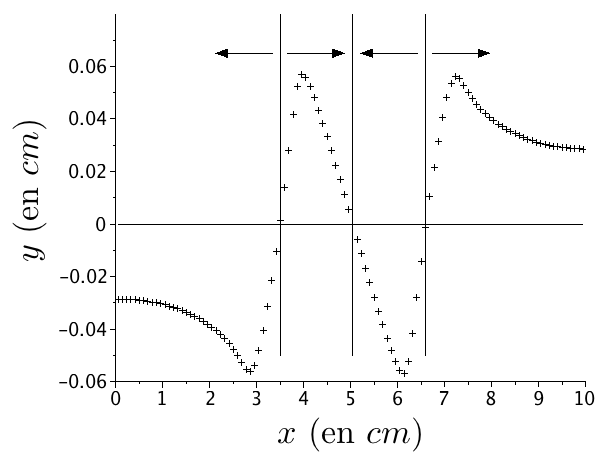
\includegraphics[width=.49\textwidth]
{track_10x10_7/coupe_vitesse_v2_56.png}
\caption{Profil de la vitesse~$\vit_x$ le long de~$\ex$ au Jour 905 -- Simulation numérique avec le modèle complet, dont la densité tumorale est présentée Figure~\ref{fig:trefle} \label{fig:vx_profile}}
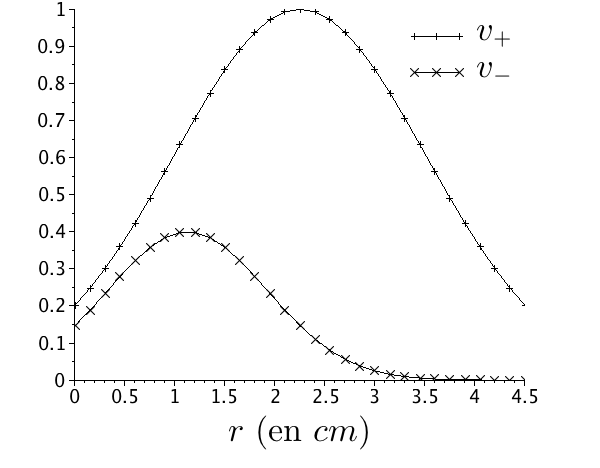
\includegraphics[width=.49\textwidth]{vitesse_imposee.png}
\caption{Composantes de la vitesse imposée dans l'équation de transport~\eqref{eq:mod_reduit_test_transp} -- Ici $L=9$ donc le rayon~$r$ varie entre~$0$ et~$4,5$\label{fig:vitesse+et-imposees} }
\end{multicols}
\end{figure}

La vitesse, que l'on impose dans l'équation~\eqref{eq:mod_reduit_test_transp}, est alors choisie comme suit en fonction du rayon~$r(\vecx)=\| \vecx - \vecx_c \|$ uniquement (le point $\vecx_c=(L/2, L/2)$ étant le centre du domaine de calcul
% de taille $L\times L$
)~:
\begin{equation}\label{eq:vit_imposee}
\vit(t,\vecx)=v\big(t,r(\vecx)\big)\frac{\vecx}{\|\vecx \|} \quad \textrm{avec} \quad v(t,r) = e^{-t} v_+(r) - \frac{t}{T_{\rm end}}v_-(r),
\end{equation}
où~$T_{\rm end}$ est le temps final de simulation (ici choisi à 1650 jours)  et où~$v_-$ et~$v_+$ sont respectivement les vitesses contractantes et dilatantes~:
\begin{align}
v_-(r)&= 0.4 \exp\left( \frac{-1}{10} \left(\frac{r-L/8}{L/8} \right)^2 \right), \label{eq:v_moins}\\
v_+(r)&=\exp\left( \frac{-1}{10} \left(\frac{r-L/4}{L/16} \right)^2 \right), \label{eq:v_plus}
\end{align}
Le profil de ces 2 vitesses est présenté à titre indicatif sur la Figure~\ref{fig:vitesse+et-imposees}. 

La vitesse imposée est donc, par construction, complètement dilatante au départ et tend vers un comportement totalement contractant en temps long. La transition s'opère avec un mélange des 2 comportements~:
\begin{myitemize}
\item dilatant en périphérie, autour d'un rayon~$L/4=2.25$,
\item contractant à l'intérieur, autour d'un rayon~$L/8=1.125$.
\end{myitemize}
Notons qu'ici la couronne dilatante ne coïncide pas avec le bord de la tumeur, puisque celle-ci est fixe~:  elle ne suit pas le front tumoral au cours du temps. 
Malgré cela, avec ce modèle extrêmement minimaliste, le trèfle à 4 feuilles apparaît lors de la simulation numérique, comme on peut le constater sur la Figure~\ref{fig:evo_test_transp}.
\begin{figure}
\centering
%\vspace{-2mm}
\subfloat[Jour 0]{\includegraphics[width=.32\textwidth,trim = 0mm 11mm 0mm 10mm, clip]{simu/test_transport/cross0/pop-001}}
\subfloat[Jour 573]{\includegraphics[width=.32\textwidth,trim = 0mm 11mm 0mm 10mm, clip]{simu/test_transport/cross0/pop-034}}
\subfloat[Jour 1010]{\includegraphics[width=.32\textwidth,trim = 0mm 11mm 0mm 10mm, clip]{simu/test_transport/cross0/pop-060}}\\
%\vspace{-2mm}
\subfloat[Jour 1179 \label{fig:evo_test_transp4}]{\includegraphics[width=.32\textwidth,trim = 0mm 11mm 0mm 10mm, clip]{simu/test_transport/cross0/pop-070}}
\subfloat[Jour 1347 \label{fig:evo_test_transp5}]{\includegraphics[width=.32\textwidth,trim = 0mm 11mm 0mm 10mm, clip]{simu/test_transport/cross0/pop-080}}
\subfloat[Jour 1499 \label{fig:evo_test_transp6}]{\includegraphics[width=.32\textwidth,trim = 0mm 11mm 0mm 10mm, clip]{simu/test_transport/cross0/pop-089}}
\caption{Evolution de la densité $P$, solution numérique du modèle réduit~\eqref{eq:mod_reduit_test_transp} (vitesse donnée par l'équation~\eqref{eq:vit_imposee}) avec un WENO5 standard -- La forme en trèfle est également visible sur le modèle réduit.\label{fig:evo_test_transp}}
\end{figure}
\begin{figure}
\centering
%\vspace{-2mm}
\subfloat[Jour 0]{\includegraphics[width=.32\textwidth,trim = 0mm 11mm 0mm 10mm, clip]{simu/test_transport/cross0.27_bis/pop-001}}
\subfloat[Jour 573]{\includegraphics[width=.32\textwidth,trim = 0mm 11mm 0mm 10mm, clip]{simu/test_transport/cross0.27_bis/pop-034}}
\subfloat[Jour 1010]{\includegraphics[width=.32\textwidth,trim = 0mm 11mm 0mm 10mm, clip]{simu/test_transport/cross0.27_bis/pop-060}}\\
%\vspace{-2mm}
\subfloat[Jour 1179]{\includegraphics[width=.32\textwidth,trim = 0mm 11mm 0mm 10mm, clip]{simu/test_transport/cross0.27_bis/pop-070}}
\subfloat[Jour 1347]{\includegraphics[width=.32\textwidth,trim = 0mm 11mm 0mm 10mm, clip]{simu/test_transport/cross0.27_bis/pop-080}}
\subfloat[Jour 1499]{\includegraphics[width=.32\textwidth,trim = 0mm 11mm 0mm 10mm, clip]{simu/test_transport/cross0.27_bis/pop-089}}
\caption{Evolution de la densité $P$, solution numérique du modèle réduit~\eqref{eq:mod_reduit_test_transp} (vitesse donnée par l'équation~\eqref{eq:vit_imposee}) avec le schéma \twinweno ($\beta=0.27$). -- Comparée à la Figure~\ref{fig:evo_test_transp}, l'invariance par rotation est ici très nettement améliorée. \label{fig:evo_test_transp_twinweno}}
\end{figure}
%Ici encore, les symptômes sont les mêmes~: on voit d'abord apparaître une altération de la forme circulaire, qui amène à un carré (\cf  Figure~\ref{fig:evo_test_transp4}), ce qui conduit ensuite  progressivement à une forme de trèfle (\cf  Figure~\ref{fig:evo_test_transp5}-\ref{fig:evo_test_transp6}).
Nous avons ainsi mis en évidence la responsabilité du schéma de transport dans l'apparition de la forme de trèfle non désirée.


\subsection{Méthode pour améliorer la préservation de l'invariance par rotation~: le \twinweno  \label{sec:twinweno}}
%De la même manière que nous avons procédé pour l'équation de Poisson, proposons un schéma pour le transport dont le stencil n'est pas uniquement réparti selon 2 directions. Le nouveau schéma, baptisé \twinweno consiste à combiner le WENO5 standard avec un autre WENO5 basé sur les directions diagonales. Ainsi l'ordre de convergence du WENO5 est préservé.\todo{ref biblio pour WENO5}
%
%Détaillons un peu plus la manière dont se présente ce schéma. Son stencil est présenté sur la Figure ...



%\subsection{Le \twinweno~: un schéma WENO5 modifié \label{sec:twinweno}}


Le schéma WENO5 standard comme donné par~\cite{Liu1994} est précis dans la plupart des cas, cependant, comme nous venons de le voir, certains ensembles de paramètres %\footnote{L'ensemble de paramètre a été trouvé par incident en  fitant l'aire tumorale de \Chen, \cf Section~\ref{section chen}.}
 produisent des instabilités numériques. De telles instabilités ont aussi été constatées avec un schéma classique upwind. 

Le problème est dû au stencil du WENO5 qui tend à favoriser les directions du maillage lors de changements de direction de la vitesse. 
Plus précisément, pour le schéma classique WENO5, en tout point 
~$\vecx_{ij}$ de la grille, l'approximation numérique 
$\W^{n+1}_{ij}$ de l'équation~\eqref{eq_transp_weno} au temps 
$t^{n+1}$ est donnée par
\begin{equation}\label{eq:WENO5}
\begin{aligned}
\W^{n+1}_{i,j}=\W^n_{i,j} + \Delta t & \Bigl(v_{i,j}^{x,n}
\mathcal{F}\left(\Delta x,(\W^n_{i+k,j})_{k=-3,\cdots, 3}\right) \\
&\quad +v_{i,j}^{y,n} \mathcal{F}\left(\Delta y,(\W^n_{i,j+k})_{k=-3,\cdots, 3}\right)\Bigr),
\end{aligned}
\end{equation}
où~$v_{i,j}^{x,n} $ et~$v_{i,j}^{y,n}$ sont définis par~\eqref{eq_vit_discr} et où~$\mathcal{F}$ est la fonction de flux WENO5 donnée par~\cite{Liu1994}. 


Pour éviter ces instabilités numériques, proposons un schéma de transport dont le stencil n'est pas uniquement réparti selon 2 directions. 
Nous introduisons un nouveau schéma, baptisé \twinweno, qui consiste en une combinaison d'un WENO5 avec son stencil standard avec un autre WENO5 dont le stencil est basé sur les directions diagonales. Cette technique aura l'avantage de conserver l'ordre de convergence élevé du WENO5, tout en améliorant considérablement son aptitude à préserver une invariance par rotation. Plus précisément, le second stencil de ce schéma est une rotation d'angle~$\ang$ du premier (\cf Figure~\ref{fig:stencil_weno5_twin}), où~$\ang$ est défini en fonction des pas d'espaces de la grille,~$\Delta x$ et~$\Delta y$, par
\begin{equation}\label{eq:angle_twinweno}
\ang=\arctan (\Delta y/\Delta x)\in (0,\pi/2).
\end{equation}
\begin{figure}[h]
  \centering
\subfloat[Grille uniforme~$\thickmuskip=1mu  \Delta x=\Delta y$]{\setlength{\unitlength}{.8mm}
\begin{picture}(65,65)
\multiput(8,8)(0,8){8}{\line(1,0){56}}
\multiput(8,8)(8,0){8}{\line(0,1){56}}
\multiput(12,12)(8,0){7}{\multiput(0,0)(0,8){7}{\circle{2}}}
\multiput(12,36)(8,0){7}{\circle*{2}}
\multiput(36,12)(0,8){7}{\circle*{2}}
\multiput(12,12)(8,8){7}{\circle*{2}}
\multiput(12,60)(8,-8){7}{\circle*{2}}
\put(8,6){\vector(1,0){8}}
\put(6,8){\vector(0,1){8}}
\put(16,6){\vector(-1,0){8}}
\put(6,16){\vector(0,-1){8}}
\put(0,11){$\Delta y$}
\put(9,2){$\Delta x$}
\end{picture}}
\subfloat[Grille non-uniforme]{\setlength{\unitlength}{.8mm}
\begin{picture}(97,65)
\multiput(8,8)(0,8){8}{\line(1,0){84}}
\multiput(8,8)(12,0){8}{\line(0,1){56}}
\multiput(14,12)(12,0){7}{\multiput(0,0)(0,8){7}{\circle{2}}}
\multiput(14,36)(12,0){7}{\circle*{2}}
\multiput(50,12)(0,8){7}{\circle*{2}}
\multiput(14,12)(12,8){7}{\circle*{2}}
\multiput(14,60)(12,-8){7}{\circle*{2}}
\put(8,6){\vector(1,0){12}}
\put(6,8){\vector(0,1){8}}
\put(20,6){\vector(-1,0){12}}
\put(6,16){\vector(0,-1){8}}
\put(0,11){$\Delta y$}
\put(9,2){$\Delta x$}
\end{picture}}
\caption{Stencil du schéma \twinweno\ pour une grille uniforme (à gauche)
  et une grille non-uniforme (à droite).} \label{fig:stencil_weno5_twin}
\end{figure} 
Nous introduisons les coefficients~$(v^{r,n}_{i,j},
v^{\theta,n}_{i,j})$ et~$\Delta r$ définis par\footnote{Les coefficients~$v^{r,n}_{i,j}$
  et~$v^{\theta,n}_{i,j}$ sont définis de sorte que 
$$\vit^n_{i,j}=v^{x,n}_{i,j}\ex+v^{y,n}_{i,j}\ey=v^{r,n}_{i,j}\er+v^{\theta,n}_{i,j}\et,\quad\text{avec}\quad 
\er=\cos\ang\,\ex+\sin\ang\,\ey,\quad \et=-\sin\ang\,\ex+\cos\ang\, \ey.$$}
\begin{equation}
\begin{pmatrix}
v^{r,n}_{i,j} \\ v^{\theta,n}_{i,j}
\end{pmatrix} = \begin{pmatrix}
\cos \ang & \sin \ang \\ -\sin \ang & \cos \ang
\end{pmatrix} \begin{pmatrix}
v^{x,n}_{i,j} \\ v^{y,n}_{i,j}
\end{pmatrix}, \qquad  \Delta r=\sqrt{\Delta x^2+\Delta y^2},
\end{equation}
et nous discrétisons l'équation~\eqref{eq_transp_weno} grâce à notre schéma \twinweno\ : 
\begin{equation}\label{eq:twin-WENO5}
  \begin{split}
\W^{n+1}_{i,j} =\W^n_{i,j} &+ (1-\beta)\Delta t \Bigl(v_{i,j}^{x,n}
\mathcal{F}\left(\Delta x,(\W^n_{i+k,j})_{k=-3,\cdots, 3}\right) \\
&\hspace{25mm} + v_{i,j}^{y,n} \mathcal{F}\left(\Delta y,(\W^n_{i,j+k})_{k=-3,\cdots,3}\right)\Bigr)\\
&+\beta\Delta t \Bigl(v_{i,j}^{r,n}
\mathcal{F}\left(\Delta r,(\W^n_{i+k,j+k})_{k=-3,\cdots, 3}\right) \\
& \hspace{25mm} + v_{i,j}^{\theta,n} \mathcal{F}\left(\Delta r,(\W^n_{i-k,j+k})_{k=-3,\cdots, 3}\right)\Bigr),
  \end{split}
\end{equation}
où~$\beta\in[0,1]$ est un paramètre numérique que nous devons choisir. 
En particulier pour~$\beta=0$, on retrouve le WENO5 standard. 


Sur la Figure~\ref{fig:evo_test_transp_twinweno}, on peut visualiser le bénéfice apporté par le \twinweno sur le modèle réduit. Ici bien que le résultat final ne soit pas parfaitement circulaire (de l'ordre de quelques pourcents d'erreur), on peut voir que la conservation de l'invariance par rotation est très améliorée. Cette amélioration est également rendue sur le modèle complet comme nous pouvons le voir sur la Figure~\ref{fig:compWENO5}, comparée à la même simulation présentée~Figure~\ref{fig:trefle}, réalisée avec un WENO5 standard.

\begin{figure}[!htb]
\centering
\subfloat[Jour 0]{\label{fig:correction_cross_spatial_1}
\includegraphics[width=0.33\textwidth]{track_14x14_cross/vue_S/1.png}}
\subfloat[Jour 543]{\label{fig:correction_cross_spatial_2}
\includegraphics[width=0.33\textwidth]{track_14x14_cross/vue_S/34.png}}
\subfloat[Jour 1053]{\label{fig:correction_cross_spatial_3}
\includegraphics[width=0.33\textwidth]{track_14x14_cross/vue_S/65.png}}
\caption{Simulation numérique avec le schéma \twinweno\  ($\beta=0.26$).  
Comparée à la Figure~\ref{fig:trefle}, la conservation de l'invariance par rotation est très clairement améliorée. 
}\label{fig:compWENO5}
\end{figure}

%\paragraph{
\subsubsection{
Quelle est la valeur optimale pour le paramètre~$\beta$ ?} 
Avec~$\beta=1$, on obtient un trèfle orienté dans les directions diagonales. 
Avec~$\beta=0.5$ aussi. Le fait que~$\Delta r$ soit supérieur à~$\Delta x$ favorise certainement la direction diagonale au détriment des autres. 
Pour l'équation~\eqref{eq:mod_reduit_test_transp} munie de la vitesse~\eqref{eq:vit_imposee}, la valeur optimale de~$\beta$ est de~$0.26$ (résultat fourni par une méthode de descente sur le paramètre~$\beta$, précis à la seconde décimale). 
Cependant cette valeur du paramètre~$\beta$, bien que faisant nettement moins apparaître le trèfle, ne semble pas être optimale pour le problème complet. 
%Pour le jeu de paramètres de la simulation présentée sur la Figure~\ref{fig:trefle}, la valeur $\beta=0.27$ est meilleure que~$0.26$. D'autres jeux de paramètres encore ont produit un optimal de~$\beta$ de~$0.3$. 
%La valeur optimale du paramètre~$\beta$ n'est donc pas transcendante~: elle ne dépend pas uniquement du schéma utilisé et des caractéristiques du maillage, mais aussi de la vitesse. L'étude du choix de ce paramètre en fonction de la vitesse n'a pas été réalisée ici. Nos simulations permettent d'en donner un encadrement~: entre~$0.2$ et~$0.4$. Ici, nous nous limiterons à~$\beta$ constant en temps, ce choix améliorant déjà de manière très satisfaisante la conservation de l'irrotationnalité.
\end{document}